\subsection{The non-equivariant adjunction (to be refactored)}
We recall the adjunction in question.
\todo[inline]{say more. come back once the paper is organized}

To extend $\tau \colon \dSet \rightleftarrows \Op \colon N$ from Definition \ref{OT_DEF} to a Quillen adjunction out of $\sOp$,
we need a topological enrichment of the inclusion $\Omega \into \Op$.
We do this by constructing the free simplicial resolution\footnote{Also called the \textit{Godement} resolution, c.f. \cite[\S 8.3]{BM06}.}
of $\Omega(T)$ as an algebra in the category of \textit{pointed} $\mathbf E(T)$-colored symmetric sequences $\Sym^{\mathbf E(T)}_{\eta}(\Set)$.
We elaborate on that distinction now.

\begin{definition}
      Given a set of colors $\mathfrak C$, let $\eta_{\mathfrak C} = \eta$ denote the initial $\mathfrak C$-colored operad in $\V$,
      defined for all $\mathfrak C$-sequences $\vect C$ by
      \[
            \eta(\vect C) =
            \begin{cases}
                  1_\V \qquad \qquad & \vect C = (x;x) \mbox{ for some $x \in \mathfrak C$,}
                  \\
                  \varnothing & \mbox{else.}
            \end{cases}
      \]
      The category of \textit{pointed} $\mathfrak C$-colored symmetric sequences in $\V$ is the category
      \[
            \Sym^{\mathfrak C}_\eta(\V) := \eta_{\mathfrak C} \downarrow \Sym^{\mathfrak C}(\V).
      \]
\end{definition}

The free operad monad $\mathbb F^{\mathfrak C}$ factors
\begin{equation}
      \label{FC_FAC_EQ}
      \begin{tikzcd}
            \Sym^{\mathfrak C}(\V) \arrow[r, shift left, "{(-) \amalg \eta}"]
            &
            \Sym^{\mathfrak C}_\eta(\V) \arrow[l, shift left] \arrow[r, shift left, "\mathbb F^{\mathfrak C}_\eta"]
            &
            \Op^{\mathfrak C}(\V) \arrow[l, shift left, "U_\eta"]
      \end{tikzcd}
\end{equation}
where the map $\eta_{\mathfrak C} \to U_\eta(\O)$ selects the identity operations for each color,
$(-) \amalg \eta$ is the (levelwise) coproduct in $\Sym^{\mathfrak C}(\V)$,
and $\mathbb F^{\mathfrak C}_\eta$ is defined on $X \in \Sym^{\mathfrak C}_\eta(\V)$ to be the pushout below computed in $\Op^{\mathfrak C}(\V)$.
\[
      \begin{tikzcd}
            \mathbb F^{\mathfrak C} \eta_{\mathfrak C} \arrow[d] \arrow[r]
            &
            \eta_{\mathfrak C} \arrow[d]
            \\
            \mathbb F^{\mathfrak C} X \arrow[r]
            &
            \mathbb F^{\mathfrak C}_\eta X
      \end{tikzcd}
\]

% The following observations are straightforward.
% \begin{lemma}
%       $\mathbb F^{\mathfrak C}_\eta$ is left adjoint to the forgetful functor $\Op^{\mathfrak C}(\V) \to \Sym^{\mathfrak C}_\eta(\V)$,
%       and \eqref{FC_FAC_EQ} is a factorization of the original free-forgetful adjunction for $\mathbb F^{\mathfrak C}$. 
% \end{lemma}

We can now make the following definition of the $W$-construction.

\begin{definition}
      Given $T \in \Omega$, define $W(T)_\bullet \in \Op(\sSet) \subseteq (\Op^{\mathbf E(T)})^{\Delta^{op}}$ to be the bar construction
      \[
            W(T)_n = \left( \mathbb F^{\mathbf E(T)}_\eta \right)^{n+1} \left(\Omega(T)\right),
      \]
      with the simplicial maps the monadic unit and monadic multiplication.
\end{definition}

We unpack this $\mathbf E(T)$-colored operad, culminating in \eqref{WT_EQ}.
First, we consider $\mathbb F^{\mathbf E(T)} \Omega(T)$ and $\mathbb F^{\mathbf E(T)}_\eta \Omega(T)$.
We observe that $\mathbb F^{\mathbf E(T)} \Omega(T)(\vect C) = \varnothing$ iff $\Omega(T)(\vect C) = \varnothing$.
Otherwise, if $C \xrightarrow{\phi} T$ is such that $\partial \phi = \vect C$, then
\begin{equation}
      \label{FET_EQ}
      \mathbb F^{\mathbf E(T)}\Omega(T)(\vect C)
      = \set{\mbox{factorizations $C \xrightarrow{\psi_0} S_1 \xrightarrow{\psi_1} T$ of $\phi$ with $\psi_0$ tall}}.
\end{equation}
We note in particular that neither map in the factorization needs to be injective;
specifically, for any $e \in \mathbf E(T)$,
\begin{equation}
      \label{FET_EE_EQ}
      \mathbb F^{\mathbf E(T)}\Omega(T)(e;e) = \mathbb Z_{\geq 0}
\end{equation}
is in bijection with the set of non-negative integers.

\begin{example}
      More generally, we consider the simple case where $T$ is the 2-corolla $C_2 \in \Sigma$, with leaves $\set{a,b}$ and root $r$.
      Then $\mathbb F^{\mathbf E(T)}\Omega(T)(a,b;r) = \mathbb Z_{\geq 0}^{\times \set{a,b,r}}$,
      where the tree $S_1$ associated to the triple $(n_a, n_b, n_r)$ has one node of valence two,
      with root (resp. left, right) path out of that node of length $n_r$ (resp. $n_a$, $n_b$).
      \[
            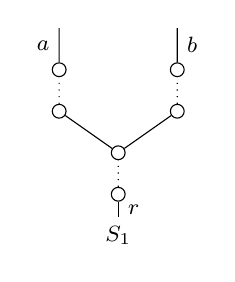
\begin{tikzpicture}
                  [grow=up,auto,
                  level distance=2em,
                  every node/.style = {font=\footnotesize,solid},
                  dummy/.style={circle,draw,inner sep=0pt,minimum size=1.75mm},
                  emph/.style={edge from parent/.style={black,thin,dotted,draw}},
                  norm/.style={edge from parent/.style={black,thin,draw,solid}}
                  ]
                  \node {$S_1$}
                  child[norm, level distance=1.5em] {node [dummy] {}
                    % child[norm, level distance=1.2em] {node [dummy] {}
                      child[emph]{node [dummy] {} % vertex
                        child[norm] {node [dummy] {}
                          child[emph] {node [dummy] {}
                            child[norm] {edge from parent node [swap] {$b$}}
                          }
                        }
                         child[norm] {node [dummy] {}
                          child[emph] {node [dummy] {}
                            child[norm] {edge from parent node {$a$}}
                          }
                        }
                      }
                      % }
                    edge from parent node [swap] {$r$}
                  };
            \end{tikzpicture}
      \]
      where there are $n_r$, $n_b$, and $n_a$ edges on the bottom, right, and left paths respectively.
\end{example}
      
Now, $\mathbb F^{\mathbf E(T)}\eta_{\mathbf E(T)}(\vect C) = \varnothing$ unless $\vect C = (e;e)$ for some $e \in \mathbf E(T)$;
in this case, $\mathbb F^{\mathbf E(T)}\eta(e;e) = \mathbb Z_{\geq 0}$, as in \eqref{FET_EE_EQ}.
% 
If we also denote the unit map by $\eta$, we see that the image of the map
\[
      \mathbb F^{\mathbf E(T)}\eta \xrightarrow{\mathbb F^{\mathbf E(T)}\eta} \mathbb F^{\mathbf E(T)} \Omega(T)
\]
corresponds to all factorizations from \eqref{FET_EQ} with $S_1$ a linear tree and $\phi$ (and hence $\psi_1$) a degeneracy.

Thus in the pushout $\mathbb F^{\mathbf E(T)}_\eta\Omega(T)$, all the non-injective operations are identified, and we have
\begin{align*}
  \mathbb F^{\mathbf E(T)}_\eta\Omega(T)(\vect C)
  & = \set{\mbox{factorizations $C \xrightarrow{\psi_0} S_1 \xrightarrow{\psi_1} T$ of $\phi$ with $\psi_1$ injective, $\psi_0$ tall}} \\
  & = \set{\mbox{inner faces $S_1$ of $T_{\phi(1 2 \dots n) \leq \phi(0)}$}} \\
  & = \set{\mbox{subsets $S_1 \subseteq \mathbf E^i(T_{\phi(1 2 \dots n) \leq \phi(0)})$ of inner edges}}    
\end{align*}
where $1 2 \dots n \leq 0$ is the vertex of $C$ and $T_{\phi(1 2 \dots n) \leq \phi(0)}$ is the associated outer face of $T$ \todo{find citation from \cite{Per18} /add discussion}.


% Iterating, we see that
% \[
%       \mathbb F(\mathbb F_\eta \Omega(T))(C)
%       = \set{
%         \begin{array}{l}
%           \mbox{factorizations $C \xrightarrow{\psi_0} S_1 \xrightarrow{\psi_1} S_2 \xrightarrow{\psi_2} T$}
%           \\
%           \mbox{of $\phi$ with $\psi_0,\psi_1$ tall and $\psi_2$ injective}
%         \end{array}
%       },
% \]
% while the image of $\eta$ in $\mathbb F_\eta \Omega(T)$ are those factorizations with
% $S_1 = \eta$,
% and the image of $\mathbb F(\eta)$ in $\mathbb F(\mathbb F_\eta \Omega(T)$ are those factorizations with
% $S_1$ linear and $S_2 = \eta$.

Inductively, we have the following:
\begin{align*}
  \left(\mathbb F^{\mathbf E(T)}_\eta \right)^{n-1} \Omega(T)(\vect C)
  & = \set{
    \begin{array}{l}
      \mbox{factorizations $C \xrightarrow{\ \quad \psi_0 \quad \ } S_1 \xrightarrow{\psi_1}
      % S_2 \xrightarrow{\psi_2}
      \dots \xrightarrow{\psi_{n-2}} S_{n-1} \xrightarrow{\psi_{n-1}} T$}
      \\
      \mbox{of $\phi$ with $\psi_i$ injective for $i > 0$ and $\psi_i$ tall for $i < n-1$}
    \end{array}
  },
  \\ % --------------------
  \mathbb F^{\mathbf E(T)} \left(\mathbb F^{\mathbf E(T)}_\eta\right)^{n-1} \Omega(T) (\vect C)
  & = \set{
    \begin{array}{l}
      \mbox{factorizations $C \xrightarrow{\psi_0} S_1 \xrightarrow{\psi_1} S_2 \xrightarrow{\psi_2} \dots \xrightarrow{\psi_{n-1}} S_n \xrightarrow{\psi_n} T$}
      \\
      \mbox{of $\phi$ with $\psi_i$ tall for $i < n$ and injective for $i > 1$}
    \end{array}
  },
  \\ % --------------------
  \mathsf{im}\left(\eta \to \left(\mathbb F^{\mathbf E(T)}_{\eta}\right)^{n-1}\Omega(T)\right)
  & = \set{
    \begin{array}{l}
      \mbox{factorizations $C_1 \xrightarrow{\ \quad \psi_0 \ \quad} \eta \xrightarrow{\psi_1}
        % \eta \xrightarrow{\psi_2}
      \dots \xrightarrow{\psi_{n-2}} \eta \xrightarrow{\psi_{n-1}} T$}
    \end{array}
  },
  \\ % --------------------
  \mathsf{im}\left(\mathbb F^{\mathbf E(T)}\left( \eta \to \left(\mathbb F^{\mathbf E(T)}_{\eta}\right)^n\Omega(T)\right)\right)
  & = \set{
    \begin{array}{l}
      \mbox{factorizations $C_1 \xrightarrow{\psi_0} S_1 \xrightarrow{\psi_1} \eta \xrightarrow{\psi_2} \dots \xrightarrow{\psi_{n-1}} \eta \xrightarrow{\psi_n} T$}
      \\
      \mbox{of $\phi$ with $S_1$ linear}
    \end{array}
  },
  \\ % --------------------
  \left(\mathbb F^{\mathbf E(T)}_\eta \right)^n \Omega(T)(\vect C)
  & = \set{
    \begin{array}{l}
      \mbox{factorizations $C \xrightarrow{\psi_0} S_1 \xrightarrow{\psi_1} S_2 \xrightarrow{\psi_2} \dots \xrightarrow{\psi_{n-1}} S_n \xrightarrow{\psi_n} T$}
      \\
      \mbox{of $\phi$ with $\psi_i$ injective for $i > 0$ and $\psi_i$ tall for $i < n$}
    \end{array}
  }
  \\
  &= \set{\mbox{nested subsets $S_1 \subseteq S_2 \subseteq \dots \subseteq S_n \subseteq \mathbf E^i(T_{\phi(1 2 \dots n) \leq \phi(0)})$}}.
  % \\
  % \left(\mathbb F^{\mathbf E(T)}\right)^n \Omega(T)(\vect C)
  % & = \set{
  %   \begin{array}{l}
  %     \mbox{factorizations $C \xrightarrow{\psi_0} S_1 \xrightarrow{\psi_1} S_2 \xrightarrow{\psi_2} \dots \xrightarrow{\psi_{n-1}} S_n \xrightarrow{\psi_n} T$}
  %     \\
  %     \mbox{of $\phi$ with $\psi_i$ tall for $i < n$}
  %   \end{array}
  % }
\end{align*}

Finally, for any finite set $A$, we recall that the $n$-simplicies of $\Delta[1]^{\times A}$ correspond to $(n+1)$-strings of nested subsets of $A$.
Thus we have the following description of $W(T)$:

\begin{equation}
      \label{WT_EQ}
      W(T)(\vect C) = 
      \begin{cases}
            \Delta[1]^{\times \mathbf E^i(T_{\underline e \leq e})}, \qquad & \mbox{there exist $C \xrightarrow{\phi} T$ with $\partial \phi = \vect C$}
            \\
            \varnothing & \text{else,}
      \end{cases}
\end{equation}

It is clear that $W(-)$ is functorial. Thus we have the following definition.
